% Auto-generated from docs/schematic/spec_units.py via render.py — edit the template, not the .tex.
\documentclass[tikz,border=6pt]{standalone}
\usepackage{amsmath}
\usepackage{tikz}
\usetikzlibrary{arrows.meta,calc}
\definecolor{predcolor}{HTML}{4C8DFF}
\definecolor{errcolor}{HTML}{E0772B}
\definecolor{valuestroke}{HTML}{222222}
\definecolor{errorstroke}{HTML}{888888}
\begin{document}
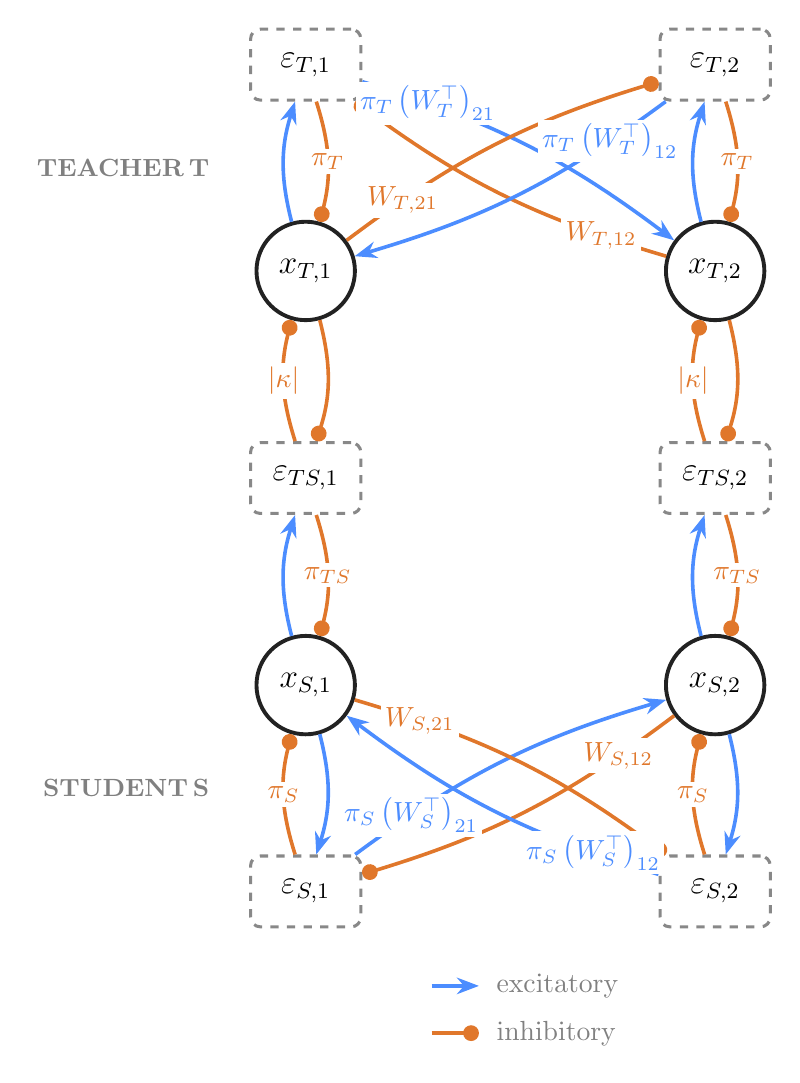
\begin{tikzpicture}[
  value/.style={circle, draw=valuestroke, line width=1.4pt, minimum size=12.5mm, inner sep=0pt, font=\large},
  error/.style={rounded corners=3.5pt, draw=errorstroke, dashed, line width=1.1pt,
                minimum width=14mm, minimum height=9mm, inner sep=2pt, font=\large},
  pred/.style={predcolor, line width=1.3pt},
  err/.style={errcolor, line width=1.3pt},
  excit/.style={-{Stealth[length=2.8mm]}},
  inhib/.style={-{Circle[length=2mm, width=2mm]}},
  glab/.style={font=\normalsize, fill=white, inner sep=1.5pt},
]
% ---- nodes ----
\node[error] (eT1) at (0.00,-0.00) {$\varepsilon_{T,1}$};
\node[value] (xT1) at (0.00,-2.62) {$x_{T,1}$};
\node[error] (eTS1) at (0.00,-5.25) {$\varepsilon_{TS,1}$};
\node[value] (xS1) at (0.00,-7.88) {$x_{S,1}$};
\node[error] (eS1) at (0.00,-10.50) {$\varepsilon_{S,1}$};
\node[error] (eT2) at (5.20,-0.00) {$\varepsilon_{T,2}$};
\node[value] (xT2) at (5.20,-2.62) {$x_{T,2}$};
\node[error] (eTS2) at (5.20,-5.25) {$\varepsilon_{TS,2}$};
\node[value] (xS2) at (5.20,-7.88) {$x_{S,2}$};
\node[error] (eS2) at (5.20,-10.50) {$\varepsilon_{S,2}$};

% ---- couplings (reciprocal pairs separate under the uniform bend) ----
\draw[pred, excit] (xT1) to[bend left=16.0] (eT1);
\draw[err, inhib] (eT1) to[bend left=16.0] node[glab, pos=0.5]{$\pi_T$} (xT1);
\draw[err, inhib] (xT1) to[bend left=16.0] (eTS1);
\draw[err, inhib] (eTS1) to[bend left=16.0] node[glab, pos=0.5]{$|\kappa|$} (xT1);
\draw[pred, excit] (xS1) to[bend left=16.0] (eTS1);
\draw[err, inhib] (eTS1) to[bend left=16.0] node[glab, pos=0.5]{$\pi_{TS}$} (xS1);
\draw[pred, excit] (xS1) to[bend left=16.0] (eS1);
\draw[err, inhib] (eS1) to[bend left=16.0] node[glab, pos=0.5]{$\pi_S$} (xS1);
\draw[pred, excit] (xT2) to[bend left=16.0] (eT2);
\draw[err, inhib] (eT2) to[bend left=16.0] node[glab, pos=0.5]{$\pi_T$} (xT2);
\draw[err, inhib] (xT2) to[bend left=16.0] (eTS2);
\draw[err, inhib] (eTS2) to[bend left=16.0] node[glab, pos=0.5]{$|\kappa|$} (xT2);
\draw[pred, excit] (xS2) to[bend left=16.0] (eTS2);
\draw[err, inhib] (eTS2) to[bend left=16.0] node[glab, pos=0.5]{$\pi_{TS}$} (xS2);
\draw[pred, excit] (xS2) to[bend left=16.0] (eS2);
\draw[err, inhib] (eS2) to[bend left=16.0] node[glab, pos=0.5]{$\pi_S$} (xS2);
\draw[err, inhib] (xT2) to[bend left=10] node[glab, pos=0.18]{$W_{T,12}$} (eT1);
\draw[pred, excit] (eT1) to[bend left=10] node[glab, pos=0.18]{$\pi_T\left(W_T^\top\right)_{21}$} (xT2);
\draw[err, inhib] (xS2) to[bend left=10] node[glab, pos=0.18]{$W_{S,12}$} (eS1);
\draw[pred, excit] (eS1) to[bend left=10] node[glab, pos=0.18]{$\pi_S\left(W_S^\top\right)_{21}$} (xS2);
\draw[err, inhib] (xT1) to[bend left=10] node[glab, pos=0.18]{$W_{T,21}$} (eT2);
\draw[pred, excit] (eT2) to[bend left=10] node[glab, pos=0.18]{$\pi_T\left(W_T^\top\right)_{12}$} (xT1);
\draw[err, inhib] (xS1) to[bend left=10] node[glab, pos=0.18]{$W_{S,21}$} (eS2);
\draw[pred, excit] (eS2) to[bend left=10] node[glab, pos=0.18]{$\pi_S\left(W_S^\top\right)_{12}$} (xS1);

% ---- population captions ----
\node[font=\small\bfseries, gray, anchor=east] at (-1.10,-1.31) {TEACHER\,T};
\node[font=\small\bfseries, gray, anchor=east] at (-1.10,-9.19) {STUDENT\,S};
% ---- legend, centred under the figure ----
\begin{scope}[shift={ (2.60,-12.10) }, font=\normalsize]
  \draw[pred, line width=1.3pt, excit] (-1, 0.4) -- ++(0.6,0);
  \node[anchor=west, gray] at (-0.3, 0.4) {excitatory};
  \draw[err, line width=1.3pt, inhib] (-1, -0.2) -- ++(0.6,0);
  \node[anchor=west, gray] at (-0.3, -0.2) {inhibitory};
\end{scope}
\end{tikzpicture}
\end{document}